\documentclass[a4paper, 12pt]{article}%тип документа

%отступы
\usepackage[left=0.6cm,right=1cm,top=2cm,bottom=3cm,bindingoffset=0cm]{geometry}
\setlength{\parindent}{5ex}

%Русский язык
\usepackage[T2A]{fontenc} %кодировка
\usepackage[utf8]{inputenc} %кодировка исходного кода
\usepackage[english,russian]{babel} %локализация и переносы

%Вставка картинок
\usepackage{graphicx}
\graphicspath{{pictures/}}
\DeclareGraphicsExtensions{.pdf,.png,.jpg}

%Графики
\usepackage{pgfplots}
\pgfplotsset{compat=1.9}

%Математика
\usepackage{amsmath, amsfonts, amssymb, amsthm, mathtools}

%Таблицы
\usepackage{longtable} 
\usepackage{float}

%Римские цифры
\newcommand{\RomanNumeralCaps}[1]{\uppercase\expandafter{\romannumeral#1}}

\usepackage{multirow}


\begin{document}
	\begin{titlepage}
		\begin{center}
			\textsc{Федеральное государственное автономное образовательное учреждение высшего образования«Московский физико-технический институт (национальный исследовательский университет)»\\[5mm]
			}
			
			\vfill
			
			\textbf{Отчёт по лабораторной работы 4.5.3 \\[3mm]
				Сканирующий интерферометр 
				\\[50mm]
			}
			
		\end{center}
		
		\hfill
		\begin{minipage}{.5\textwidth}
			Выполнил студент:\\[2mm]
			Сериков Алексей Романович\\[2mm]
			группа: Б03-103\\[5mm]
			
		\end{minipage}
		\vfill
		\begin{center}
			Москва, 2023 г.
		\end{center}
		
	\end{titlepage}
	
	\newpage
	\textbf{Аннотация}\\
	
	
	\textbf{Цель работы: }\\
	
	Знакомство с устройством и работой газового лазера
	непрерывного действия, со спектральными характеристиками лазерного излучения, а также с устройством и принципом действия сканирующего интерферометра Фабри–Перо.\\
	
	\textbf{В работе используются: }\\
	
	Не-Nе лазер с блоком питания; сканирующий интерферометр Фабри–Перо; поляроид; пластинка $\lambda / 4$; линза;
	фотодиод; электронный осциллограф.\\
	
	\textbf{Теоретическая справка:}\\
	
	
	
	\noindent \textbf{Устройство He-Ne-лазера.}\\
	
	Основным элементом Hе-Ne лазера непрерывного действия
	является газоразрядная трубка
	Т (рис. 1).
	
	\begin{figure}[H]
		\begin{center}
				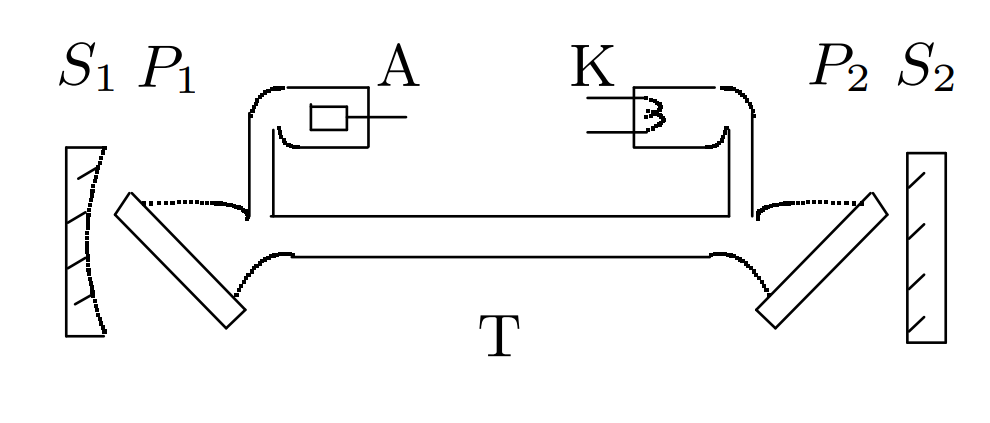
\includegraphics[width=0.3\textwidth]{Лазер.png}
			\caption{Устройство гелий-неонового лазера}
		\end{center}
	\end{figure}

	Трубка наполнена смесью гелия и неона. Концы трубки закрыты плоскопараллельными стеклянными или кварцевыми пластинами P1 и P2, установленными под углом
	Брюстера к ее оси. Линейно поляризованный свет с электрическим
	вектором, лежащим в плоскости падения, не испытывает потерь на
	отражение, вследствие этого лазер генерирует линейно поляризованное излучение. В загнутых концах трубки располагаются анод А и
	катод К. Разряд в трубке возникает при напряжении 1,5–2 кВ. Трубка помещена между зеркалами S1 и S2, образующими интерферометр
	Фабри–Перо, который играет роль оптического резонатора.
	
	
	В интерферометрах Фабри–Перо, используемых в лазерах, излучение распространяется вдоль оси интерферометра. Если на полном оптическом пути $2L$, где $L$ — расстояние между зеркалами, укладывается целое число длин волн, наступает резонанс. Условие резонанса имеет вид:
	
	
	\begin{equation}
		2L = m \lambda.
	\end{equation}
m - целое число.

Различным значениям порядка интерференции m соответствуют стоячие волны разных частот. Их называют типами колебаний, или модами. Из (1) легко получить выражение для межмодового расстояния $\Delta \nu$(в единицах частоты):
\begin{equation}
	\Delta \nu = \frac{c}{2L}.
\end{equation}
	c - скорость света.
	
	
	\noindent \textbf{Сканирующий интерферометр.}\\
	
	В работе используется сканирующий интерферометр, представляющий собой высокодобротный интерферометр Фабри–Перо с периодически изменяемой базой. Его	устройство схематически показано на рис. 2.
	
	
	\begin{figure}[H]
		\begin{center}
			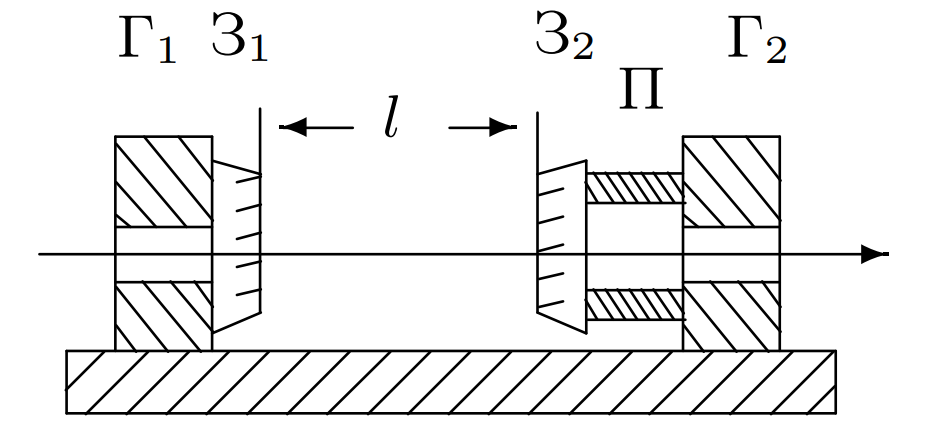
\includegraphics[width=0.3\textwidth]{Ф-П.png}
			\caption{Устройство сканирующего интерферометра}
		\end{center}
	\end{figure}
	
	Если вдоль оси интерферометра распространяется световое излучение с длиной волны $\lambda$, то при выполнении условия
	
	\begin{equation}
		2l = m \lambda.
	\end{equation}
	m - целое число, аналогичного условию (1) для лазера, возникает резонанс
	
	Собственные моды интерферометра отличаются по частоте на величину
	
	\begin{equation}
		\Delta f = \frac{c}{2l}.
	\end{equation}

Величина $\Delta f$ называется дисперсионной областью спектрального прибора. В единицах $\lambda$ дисперсионная область сканирующего интерферометра равна
	
	
		\begin{equation}
		\Delta \lambda_\text{СИ} = \frac{\lambda}{m} = \frac{\lambda ^ 2}{2l}.
	\end{equation}
	
	В нашей работе интерферометр Фабри–Перо используется как спектральный прибор высокой разрешающей силы. Разрешающая способность $R$ спектрального прибора определяется отношением
	
	\begin{equation}
		R = \frac{\lambda}{\delta \lambda}.
	\end{equation}
	
	
	где $\delta \lambda$ — минимальная разность длин волн, разрешимая прибором вблизи длины волны $\lambda$. Или
	
		\begin{equation}
		\Delta f = \nu \frac{\delta\lambda}{\lambda} = \frac{c (1- r)}{2\pi l}.
	\end{equation}
	
	
	
	При определении $\delta \lambda$ обычно используют критерий разрешения Релея. Разрешающая способность интерферометра Фабри–Перо зависит от длины интерферометра $l$ и
	коэффициента отражения зеркал $r$:
	
	\begin{equation}
		R = \frac{2 \pi l}{\lambda(1 - r)}.
	\end{equation}
	
	\newpage 
	
	
	
	
	
	\textbf{Ход работы и обработка результатов.}\\
	
1.	Рассчитаем межмодовое расстояние резонатора ОКГ в единицах $\nu$ и
	$\lambda$, используя формулу (2). Длина лазера L = 65 см ; $\lambda$ =
	= $632.8 $ нм.\\
	
	
2. Сосчитав число промежутков между модами на экране, оценим видимую ширину спектральной линии неона $\Delta\lambda(Ne)$:


Полагая, что ширина спектральной линии обусловлена эффектом
Доплера и что видимая ширина линии неона порядка полуширины доплеровского контура ($\Delta\lambda(Ne) \approx \Delta\lambda_D$), оцените среднюю скорость атомов неона vx и газокинетическую температуру T в разряде:


\begin{equation}
	\frac{\Delta\lambda_D}{\lambda} \simeq \frac{v_x}{c}.
\end{equation}

\begin{equation}
	\frac{mv_x^2}{2} \simeq \frac{kT}{2}.
\end{equation}

Здесь $v_x$ — скорость молекул неона вдоль оси лазера; $m_{Ne}$ = 20,2 а. е. м.;
1 а. е. м. = 1,66 · $10^{-24} $г.\\


3.Рассчитаем дисперсионную область $\Delta \lambda_\text{СИ}$ сканирующего интерферометра по формуле (4) для $l$ = 9 см и сравним её с видимой шириной
линии неона $\Delta\lambda(Ne)$.\\

4. Сравнив ширину отдельной моды на полувысоте с межмодовым расстоянием, оценим разрешение $\delta\lambda$ сканирующего интерферометра и разрешающую способность $R$ по формуле (5).
Оценим коэффициент отражения зеркал интерферометра $r$ по формуле (6).\\

Приведем результаты в таблице ниже:

	\begin{longtable}{|c|c|c|c|c|c|c|c|c|}
		\hline
		$\Delta\lambda$, нм& $\Delta\nu$, МГц&  $\Delta\lambda(Ne)$, нм& $v_x$, м/с& T, K& $\Delta \lambda_\text{СИ}$, нм&$\delta\lambda$, нм& R&r \\ \hline
		3.08 $\cdot 10 ^{-4}$ &  230 & 9.24 $\cdot 10 ^{-4}$&  435 &  515 & 3515& 0.44 $\cdot 10 ^{-4}$ & 145 $\cdot 10 ^{4}$& $\approx 1$ \\ \hline
		
		\caption{Таблица с результатами подсчёта.}
	\end{longtable}
	
	На рис.3 график с осциллографа.
 
	
	\begin{figure}[H]
		\begin{center}
			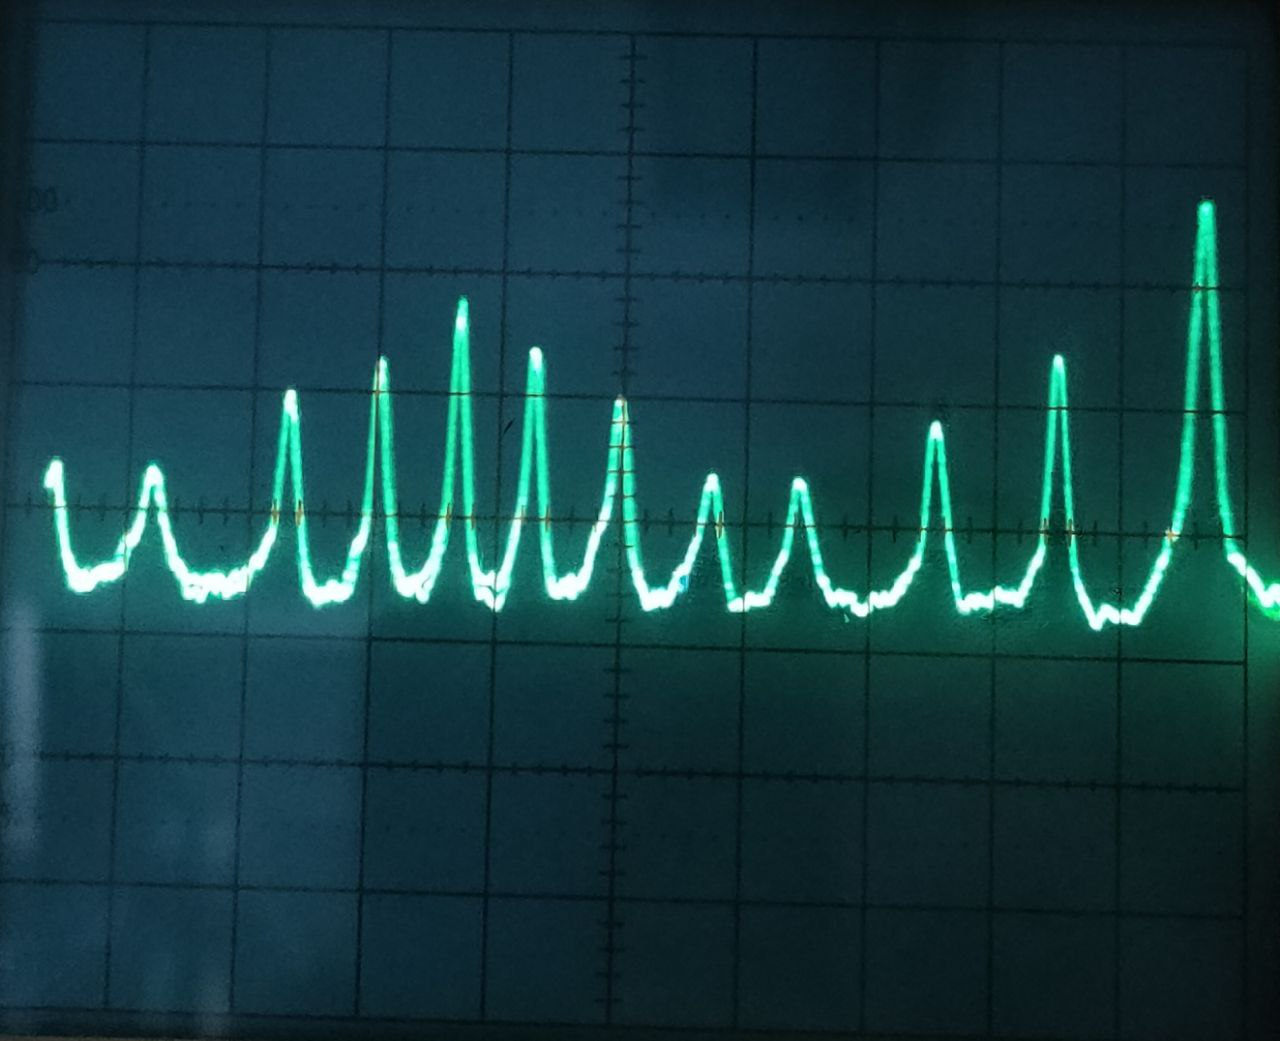
\includegraphics[width=0.4\textwidth]{Спектр.jpg}
			\caption{Данные с осциллографа}
		\end{center}
	\end{figure}

	
	\textbf{Обсуждение результатов и выводы: }\\
	В работе мы исследовали доплеровский контур спектральной линии: определили межмодовое расстояние и приборную ширину отдельной моды излучения лазера; оценили газокинетическую температуру в разряде; рассчитали дисперсионную область, разрешающую способность и коэффициент отражения зеркал сканирующего интерферометра. Результаты схожи с табличными данными.
	
	
	
\end{document}